% Chapter 1

\chapter{Simulation Results} % Write in your own chapter title
\label{Chapter5}
\lhead{Chapter 5. \emph{Simulation Results}} % Write in your own chapter title to set the page header
\section{Gate Signals}
The Gating Signals applied to both H bridges in order to get 9 levels in output voltage waveform is shown blow. Because the Input DC Source was unequal so we have to define specific sequences for all switches. The Conduction Angles are listed here:
\begin{center}
	\begin{tabular}{ |p{4cm}||p{4cm}|  }
		\hline
		\multicolumn{2}{|c|}{Conduction Angles} \\
		\hline
		Angle & Value in Degrees\\
		\hline
		$\alpha1$ & 6$^o$\\
		\hline
		$\alpha2$ & 22$^o$\\
		\hline
		$\alpha3$ & 38$^o$\\
		\hline
		$\alpha4$ & 60$^o$\\
		\hline
	\end{tabular}
\end{center}

\begin{figure}[htbp]
	\centering
	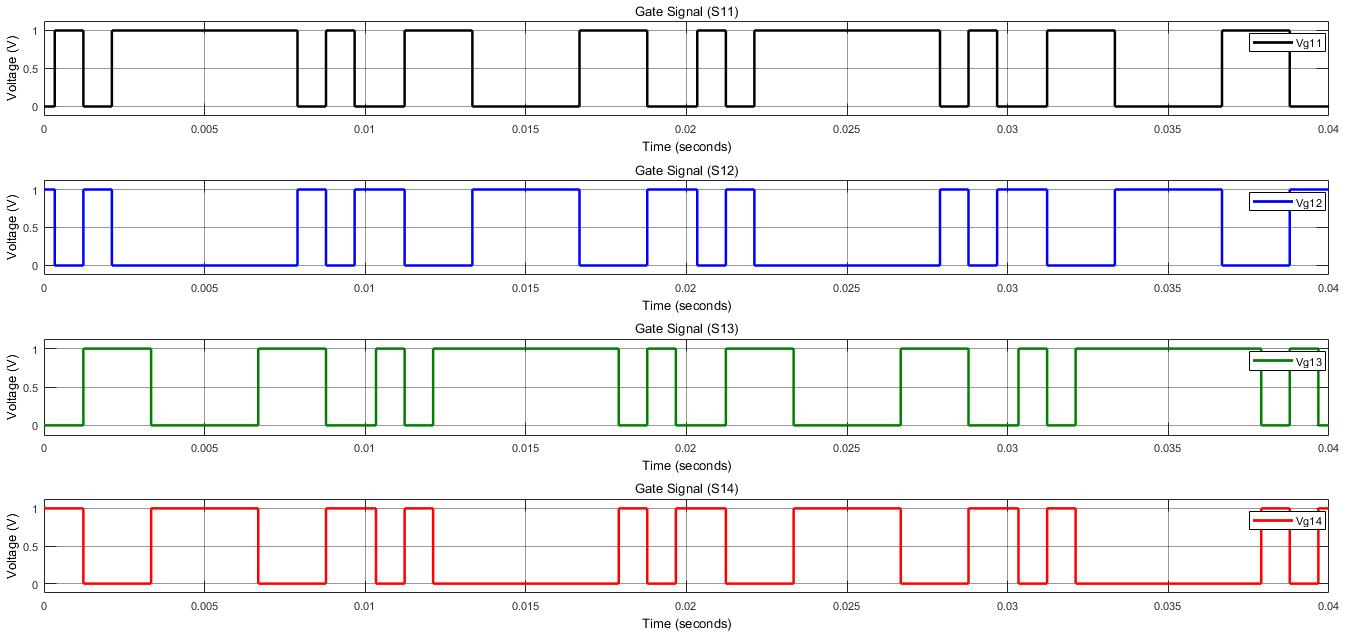
\includegraphics[width = 6in]{./Figures/Photos/Simulink/GateSignal1.jpg}
	\rule{35em}{1pt}
	\caption{Gate Signals to H-Bridge 1}
\end{figure}

\begin{figure}[htbp]
	\centering
	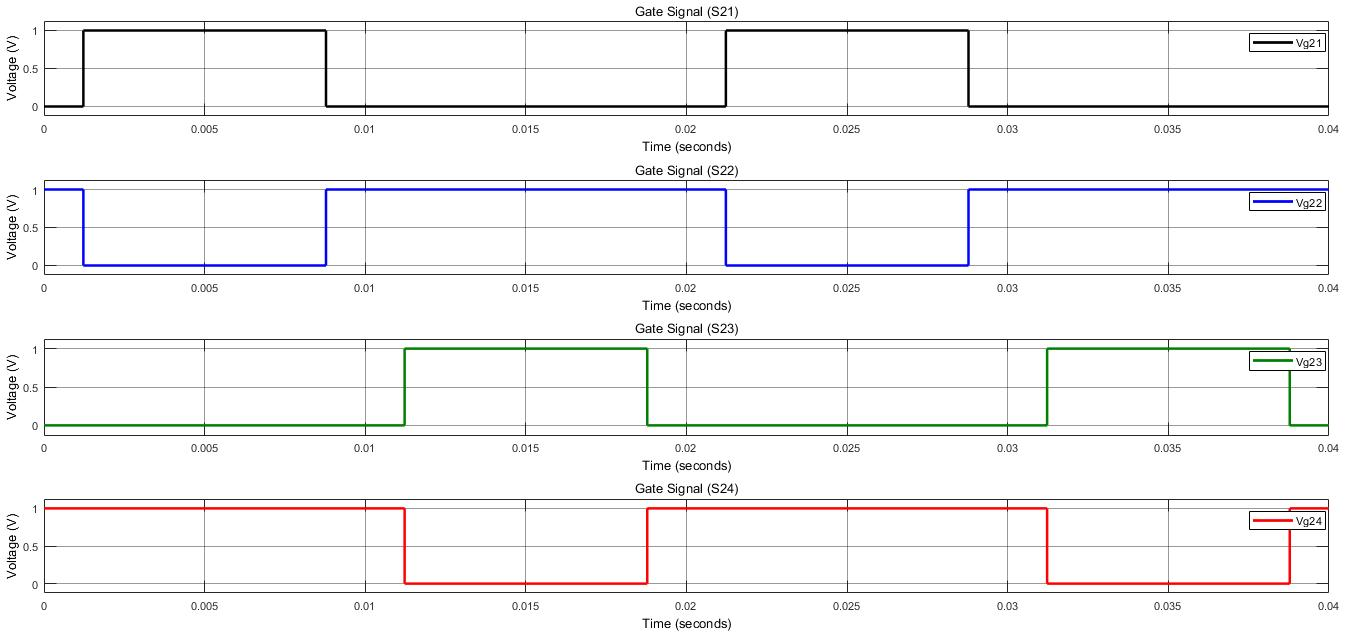
\includegraphics[width = 6in]{./Figures/Photos/Simulink/GateSignal2.jpg}
	\rule{35em}{1pt}
	\caption{Gate Signals to H-Bridge 2}
\end{figure}

\section{Source Currents}
Below is the display of source currents when Resistive load is used:
\begin{figure}[htbp]
	\centering
	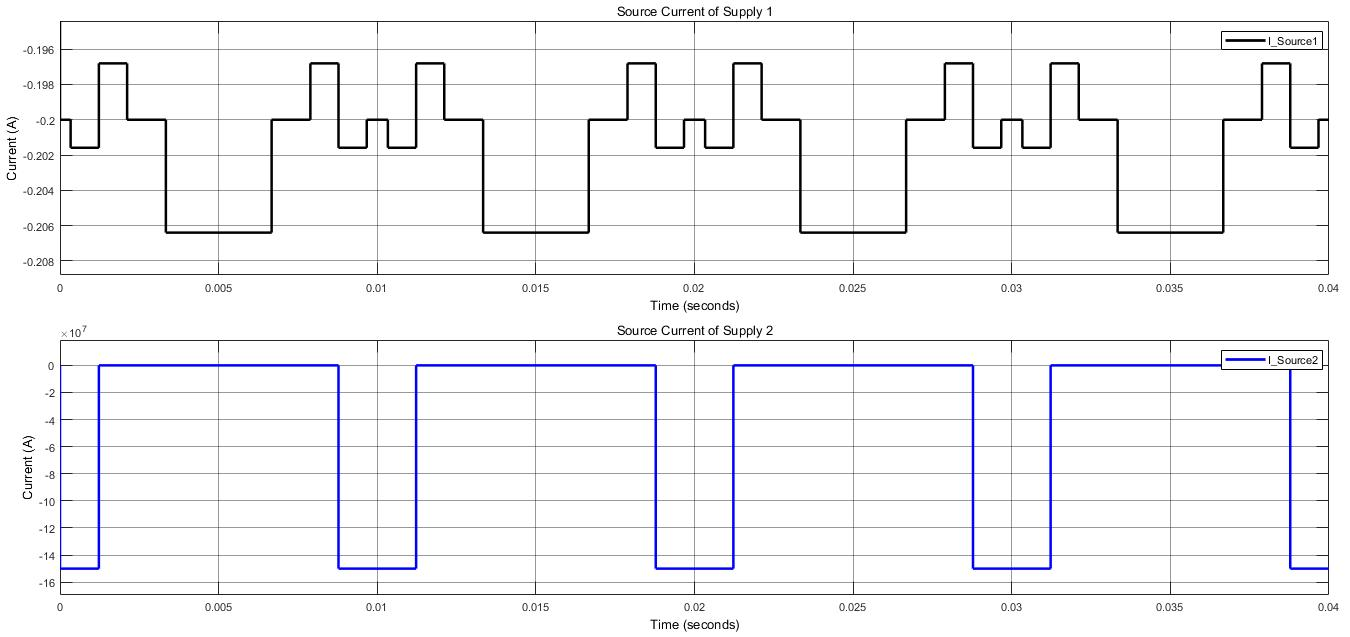
\includegraphics[width = 6in]{./Figures/Photos/Simulink/Source_Current_Res.jpg}
	\rule{35em}{1pt}
	\caption{Source Currents (Resistive Load)}
\end{figure}
\newpage
Below is the display of source currents when Resistive plus Inductive load is used at 0.8 power Factor:
\begin{figure}[htbp]
	\centering
	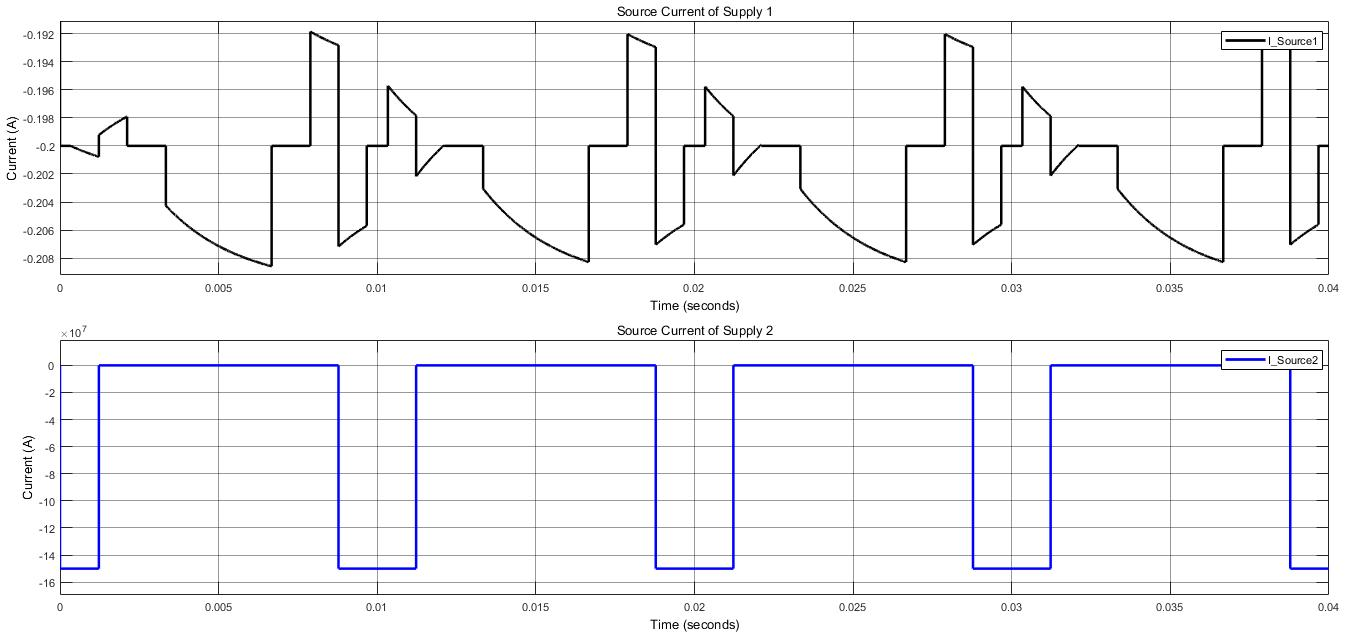
\includegraphics[width = 6in]{./Figures/Photos/Simulink/Source_Current_Induc.jpg}
	\rule{35em}{1pt}
	\caption{Source Currents (Inductive Load 0.8PF)}
\end{figure}

\section{Switch Currents}
Below is the display of switch currents when Resistive load is used:
\begin{figure}[htbp]
	\centering
	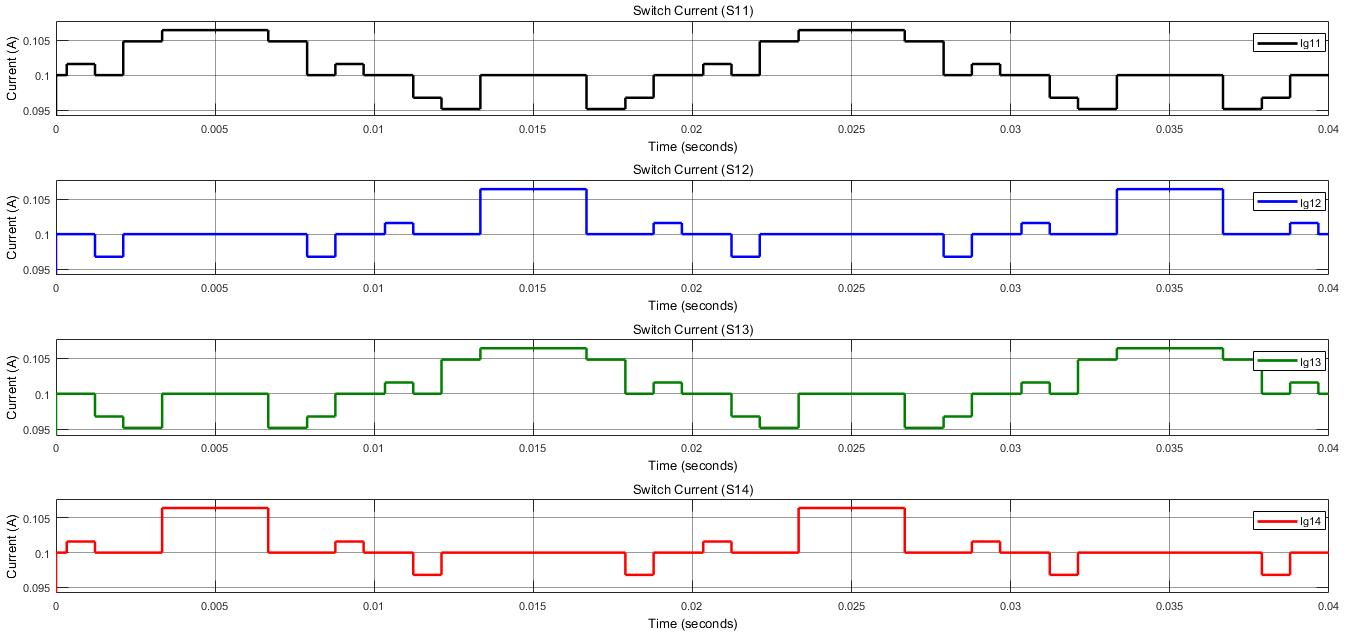
\includegraphics[width = 6in]{./Figures/Photos/Simulink/Switch_currents_1_Res.jpg}
	\rule{35em}{1pt}
	\caption{Switch Currents of H-Bridge 1 (Resistive Load)}
\end{figure}

\begin{figure}[htbp]
	\centering
	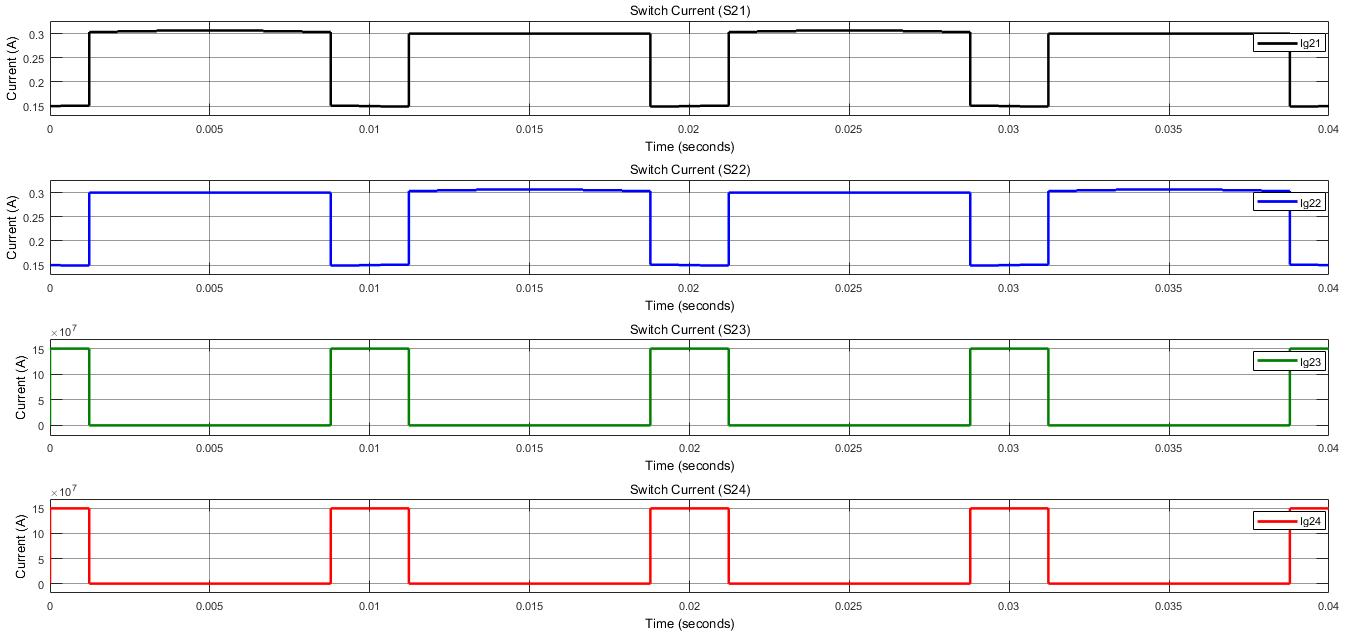
\includegraphics[width = 6in]{./Figures/Photos/Simulink/Switch_currents_2_Res.jpg}
	\rule{35em}{1pt}
	\caption{Switch Currents of H-Bridge 2 (Resistive Load)}
\end{figure}
\newpage
Below is the display of switch currents when Resistive plus Inductive load is used at 0.8 power factor:
\begin{figure}[htbp]
	\centering
	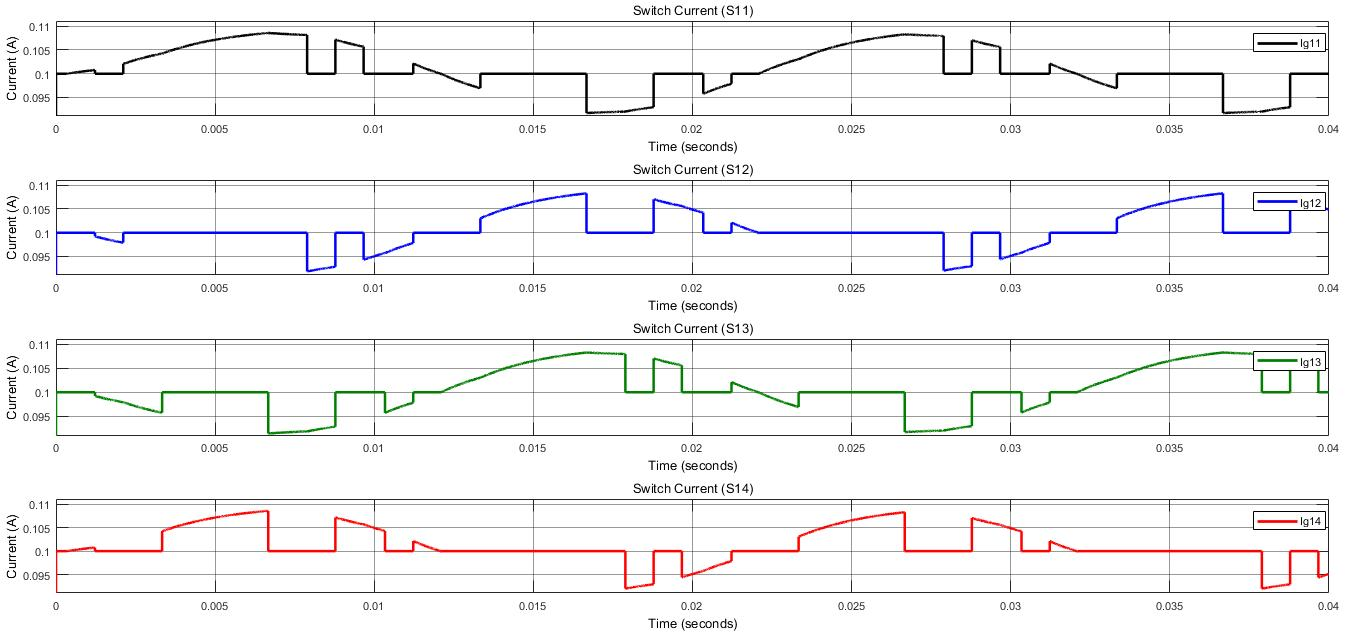
\includegraphics[width = 6in]{./Figures/Photos/Simulink/Switch_currents_1_Induc.jpg}
	\rule{35em}{1pt}
	\caption{Switch Currents of H-Bridge 1 (Inductive Load 0.8PF)}
\end{figure}

\begin{figure}[htbp]
	\centering
	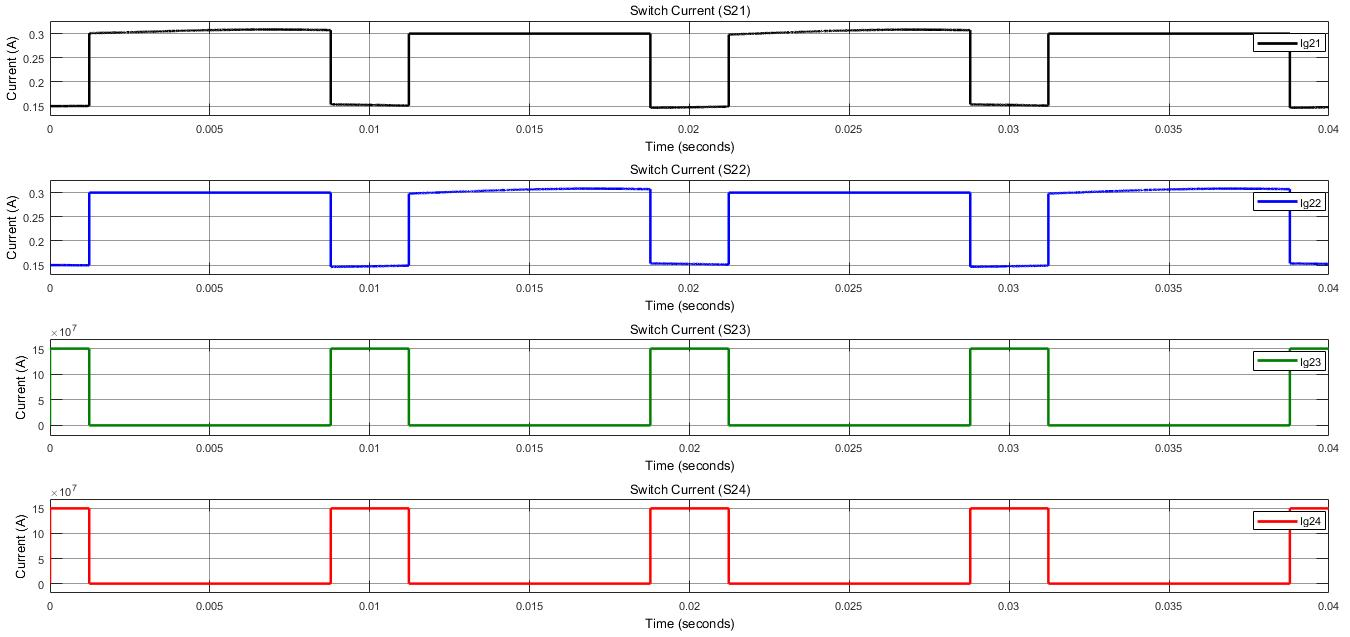
\includegraphics[width = 6in]{./Figures/Photos/Simulink/Switch_currents_2_Induc.jpg}
	\rule{35em}{1pt}
	\caption{Switch Currents of H-Bridge 2 (Inductive Load 0.8PF)}
\end{figure}
\newpage
\section{Load Current}
Load Current waveform when resistive load is used:
\begin{figure}[htbp]
	\centering
	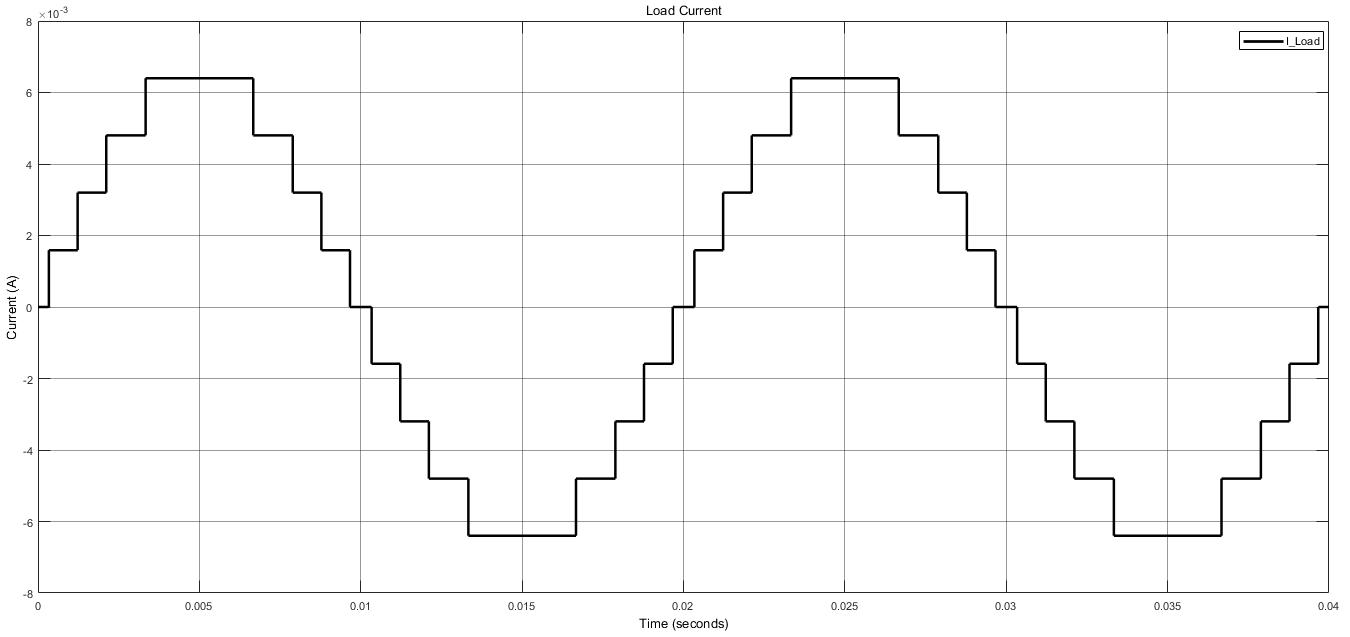
\includegraphics[width = 6in]{./Figures/Photos/Simulink/Load_Current_Res.jpg}
	\rule{35em}{1pt}
	\caption{Load Current (Resistive Load)}
\end{figure}
Below is the display of load current when Resistive plus Inductive load is used at 0.8 power factor:
\begin{figure}[htbp]
	\centering
	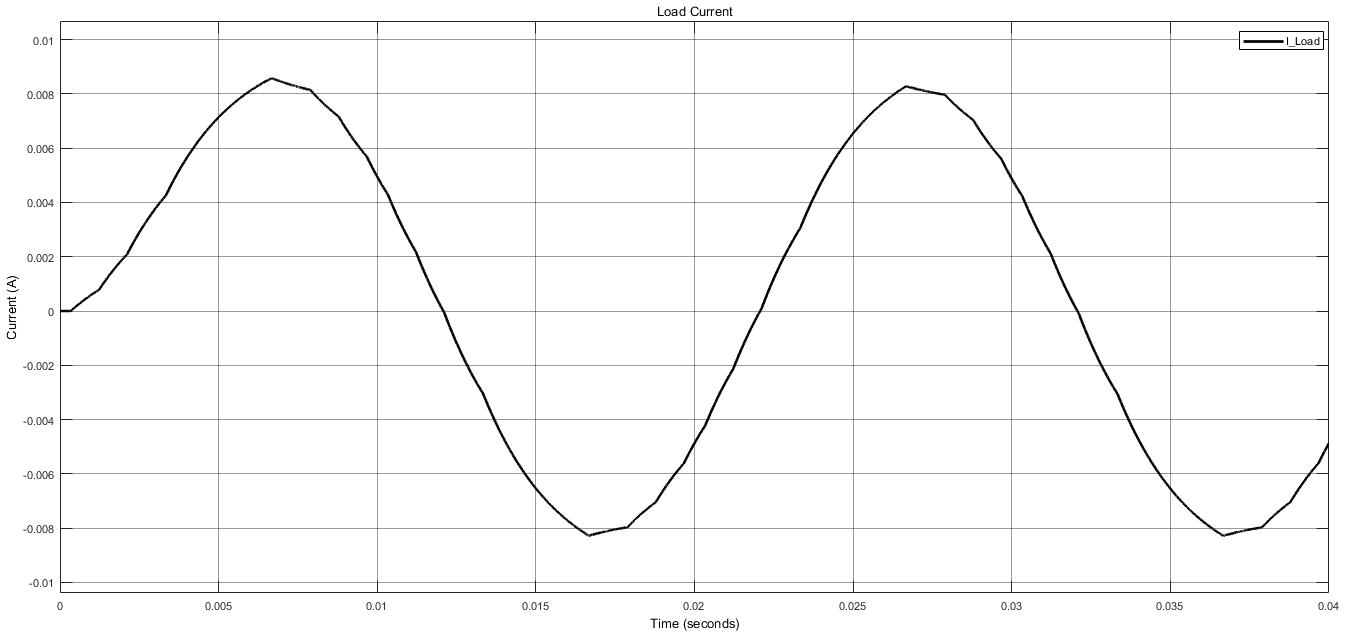
\includegraphics[width = 6in]{./Figures/Photos/Simulink/Load_Current_Induc.jpg}
	\rule{35em}{1pt}
	\caption{Load Current (Inductive Load 0.8PF)}
\end{figure}

\begin{figure}[htbp]
	\centering
	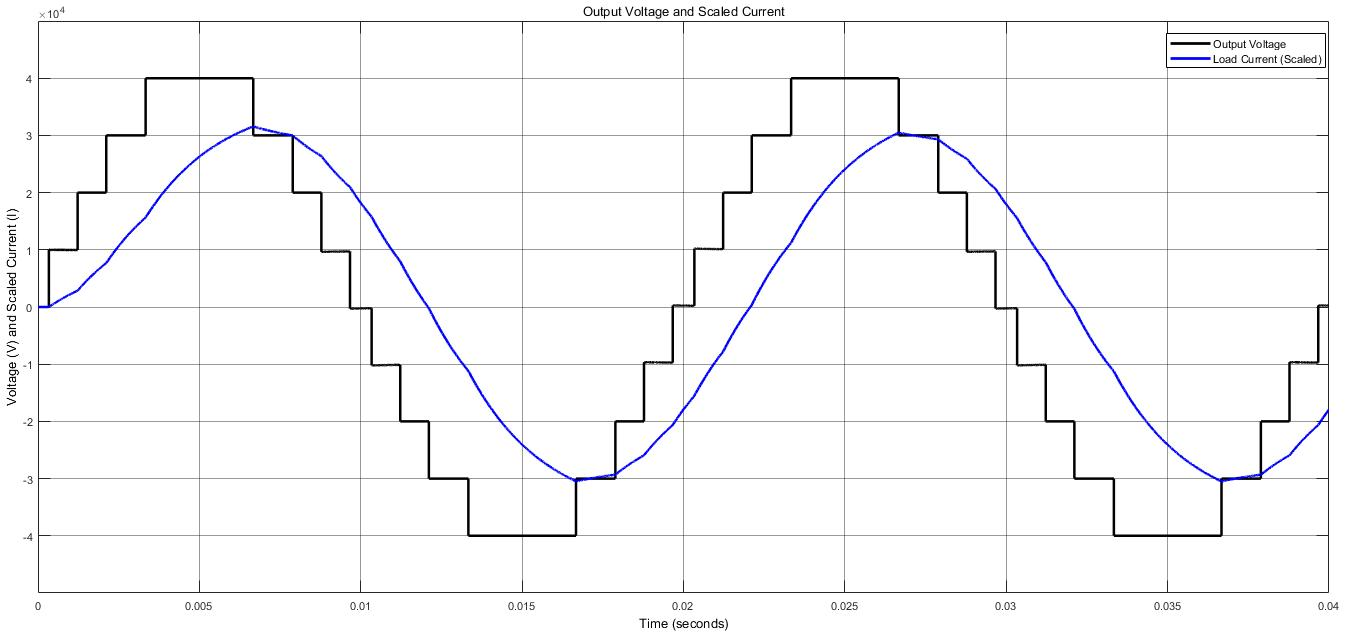
\includegraphics[width = 6in]{./Figures/Photos/Simulink/Load_Voltage_Current_Induc.jpg}
	\rule{35em}{1pt}
	\caption{Load Voltage and Scaled Current (Inductive Load 0.8PF)}
\end{figure}
\newpage
\section{Output Voltage}
The output voltage and its FFT analysis is shown below:
\begin{figure}[htbp]
	\centering
	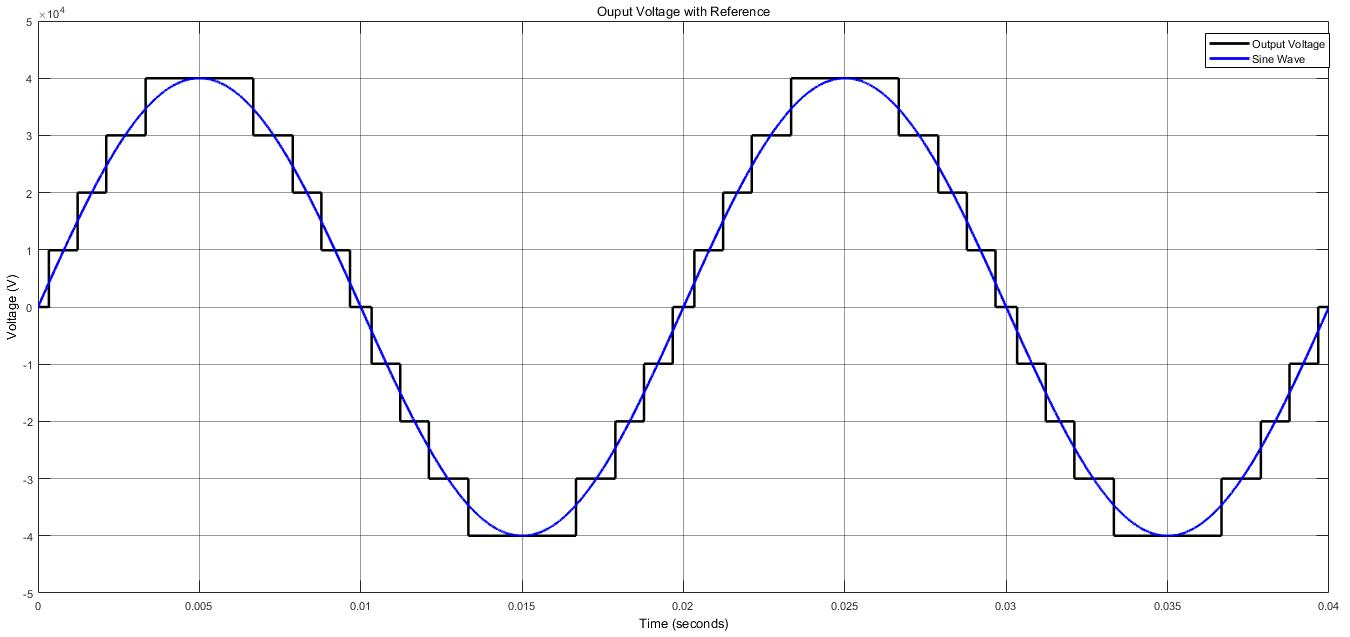
\includegraphics[width = 6in]{./Figures/Photos/Simulink/Output.jpg}
	\rule{35em}{1pt}
	\caption{Output Voltage}
\end{figure}
\begin{figure}[htbp]
	\centering
	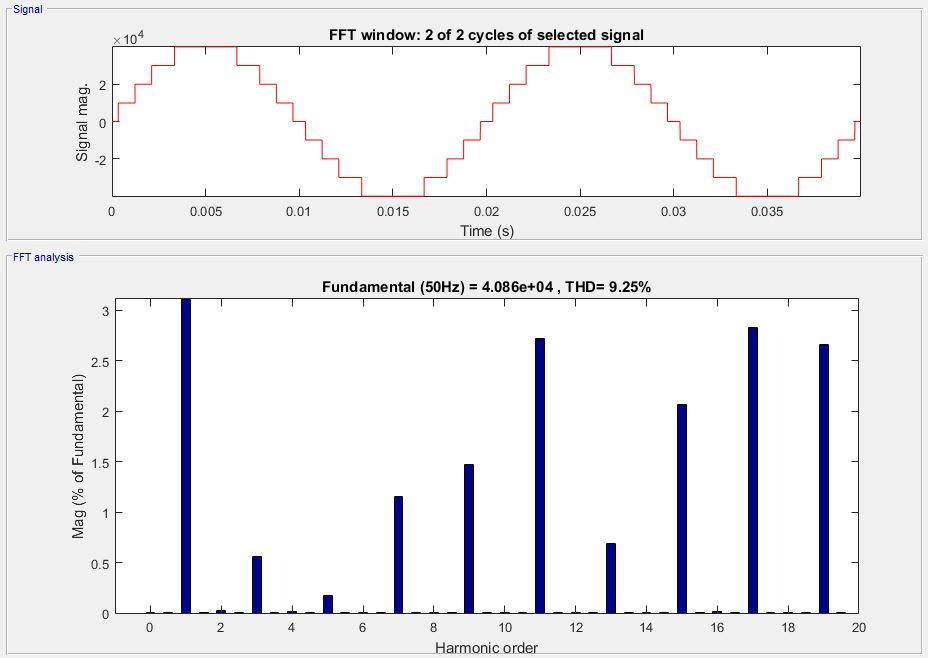
\includegraphics[width = 6in]{./Figures/Photos/Simulink/Output_FFT.jpg}
	\rule{35em}{1pt}
	\caption{Output Voltage FFT Analysis}
\end{figure}
\begin{figure}[htbp]
	\centering
	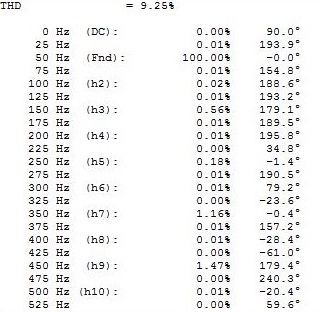
\includegraphics[width = 4in]{./Figures/Photos/Simulink/Output_FFT_tab.jpg}
	\rule{35em}{1pt}
	\caption{Record of First 10 Harmonics}
\end{figure}
\newpage

\section{Output Generated by PWM Technique}
The output voltage generated by programming based PWM technique is shown below, the switch frequency is 10kHz and duty is 50 percent.
\begin{figure}[htbp]
	\centering
	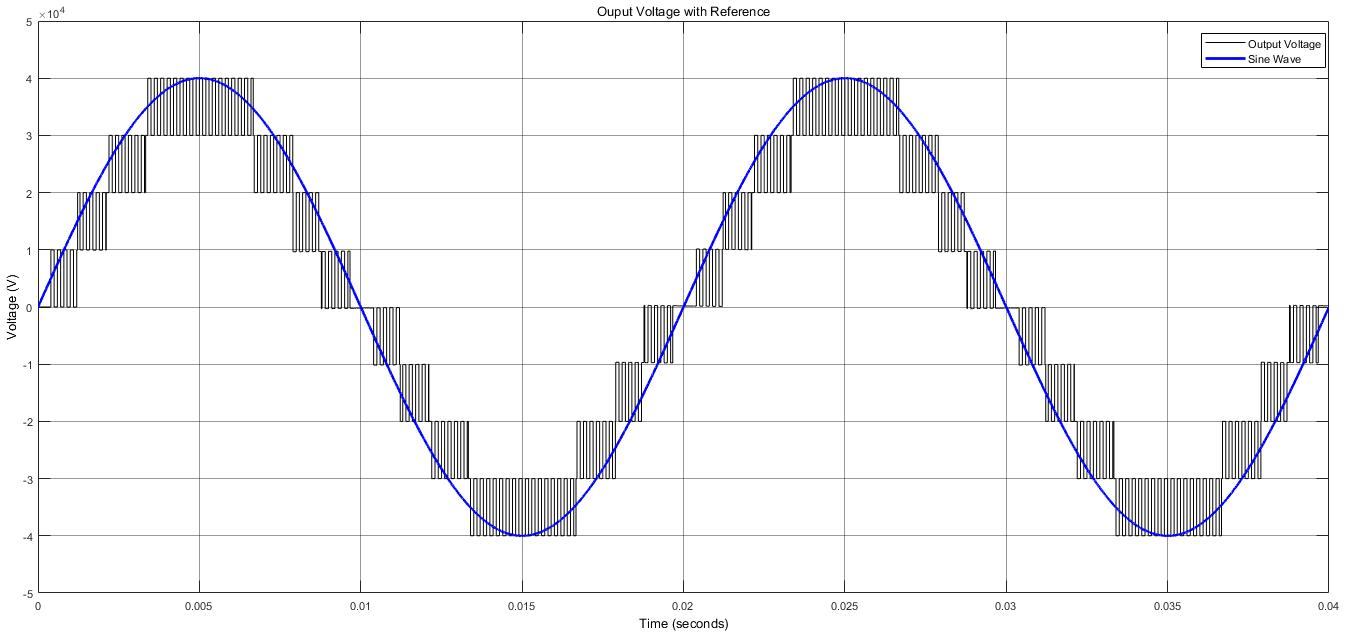
\includegraphics[width = 6in]{./Figures/Photos/Simulink/PWM_Out.jpg}
	\rule{35em}{1pt}
	\caption{Output Signal Generated by PWM Technique}
\end{figure}

\begin{figure}[htbp]
	\centering
	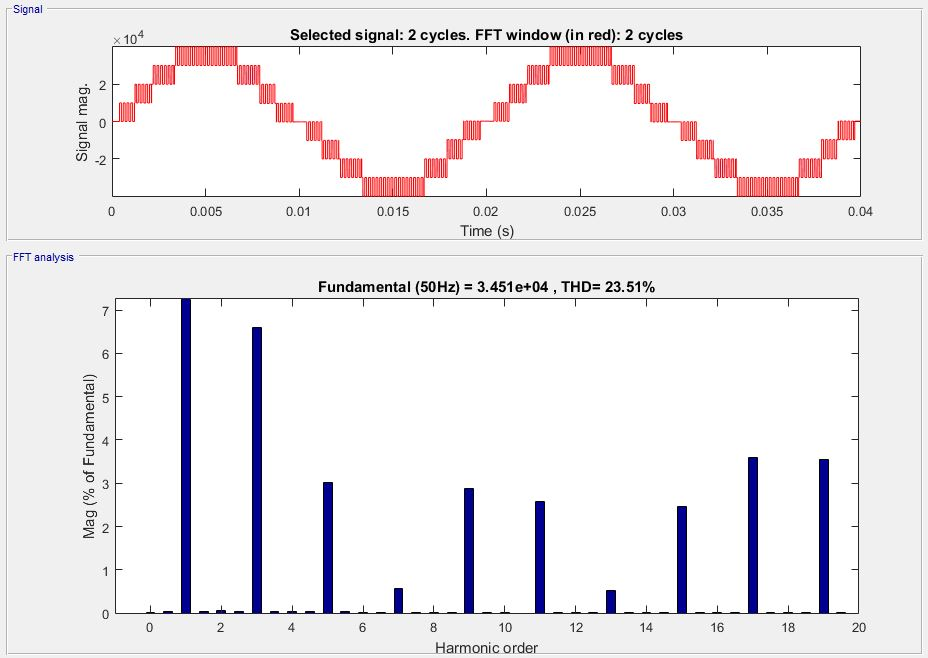
\includegraphics[width = 6in]{./Figures/Photos/Simulink/PWM_Out_FFT.jpg}
	\rule{35em}{1pt}
	\caption{FFT of Output Signal Generated by PWM Technique}
\end{figure}

\section{Output Generated by Sine PWM Technique}
The output voltage generated by programming based PWM technique is shown below, the switch frequency is 10kHz, m$_f$ is 200 and m$_a$ is 0.8.
\begin{figure}[htbp]
	\centering
	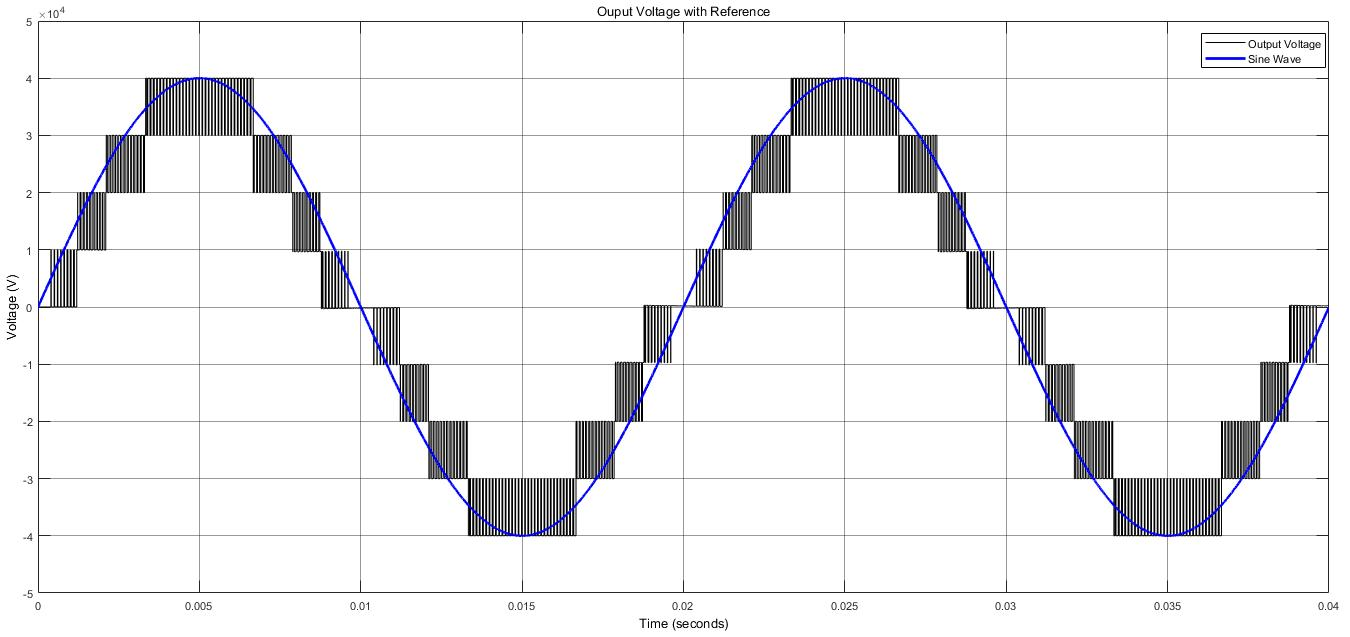
\includegraphics[width = 6in]{./Figures/Photos/Simulink/SPWM_Out.jpg}
	\rule{35em}{1pt}
	\caption{Output Signal Generated by Sine PWM Technique}
\end{figure}

\begin{figure}[htbp]
	\centering
	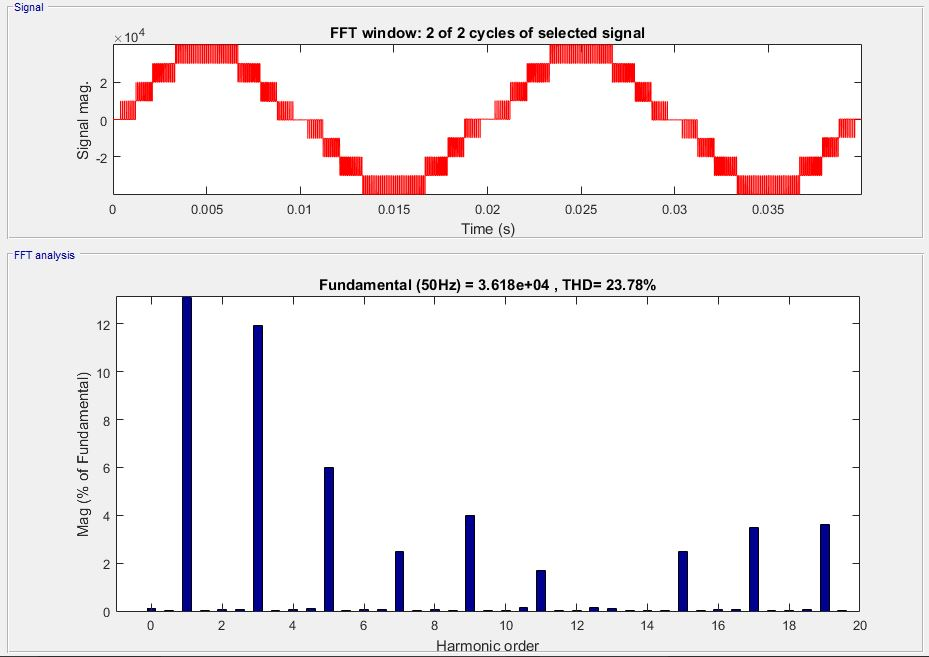
\includegraphics[width = 6in]{./Figures/Photos/Simulink/SPWM_Out_FFT.jpg}
	\rule{35em}{1pt}
	\caption{FFT of Output Signal Generated by Sine PWM Technique}
\end{figure}

\section{AND Operation with PWM Signal}
A PWM Signal of 10kHz frequency is generated and AND operation is performed with all gating signals, the output is shown below:
\begin{figure}[htbp]
	\centering
	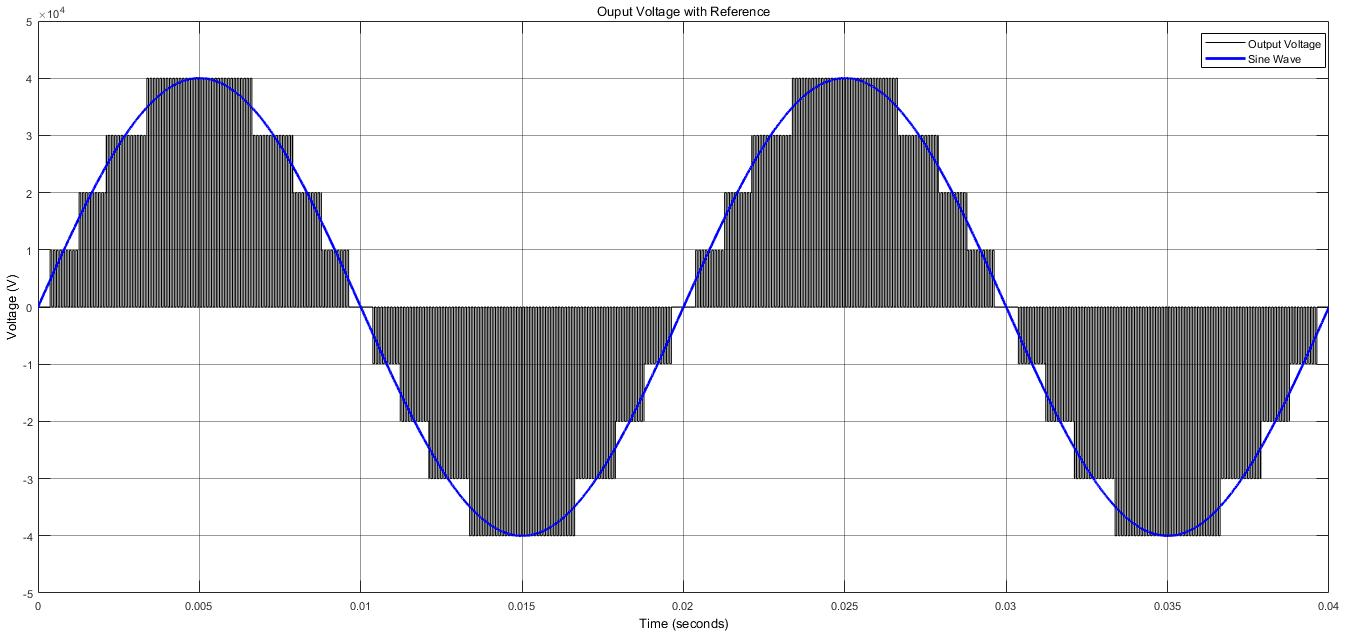
\includegraphics[width = 6in]{./Figures/Photos/Simulink/And_PWM_Out.jpg}
	\rule{35em}{1pt}
	\caption{Output Signal after AND Operation}
\end{figure}

\begin{figure}[htbp]
	\centering
	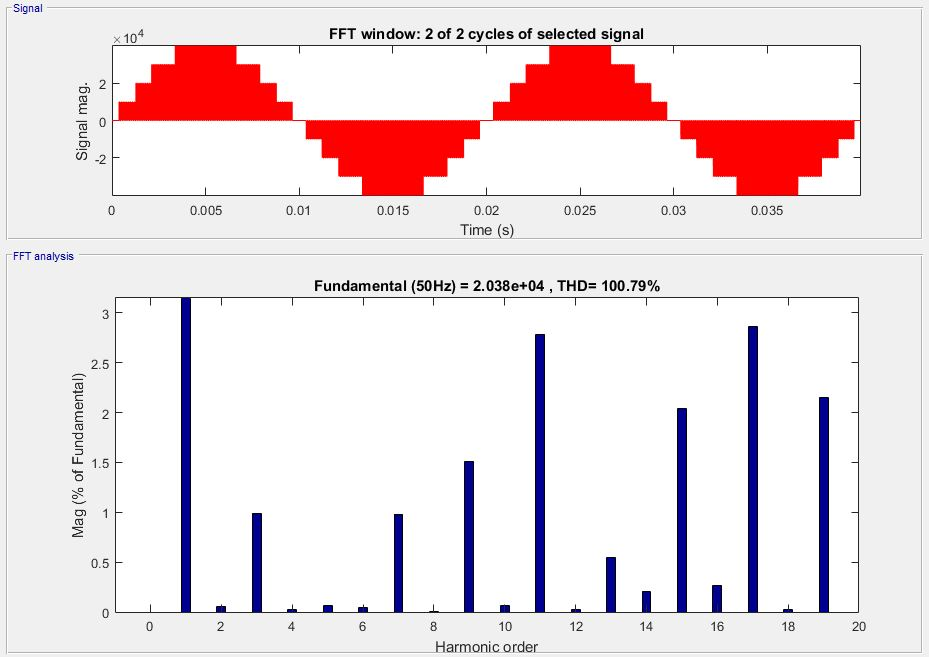
\includegraphics[width = 6in]{./Figures/Photos/Simulink/And_PWM_Out_FFT.jpg}
	\rule{35em}{1pt}
	\caption{FFT of Output Signal after AND Operation}
\end{figure}

\section{AND Operation with Sine PWM Signal}
A Sine PWM Signal of 200 m$_f$ and 0.8 m$_a$ is generated and AND operation is performed with all gating signals, the output is shown below:
\begin{figure}[htbp]
	\centering
	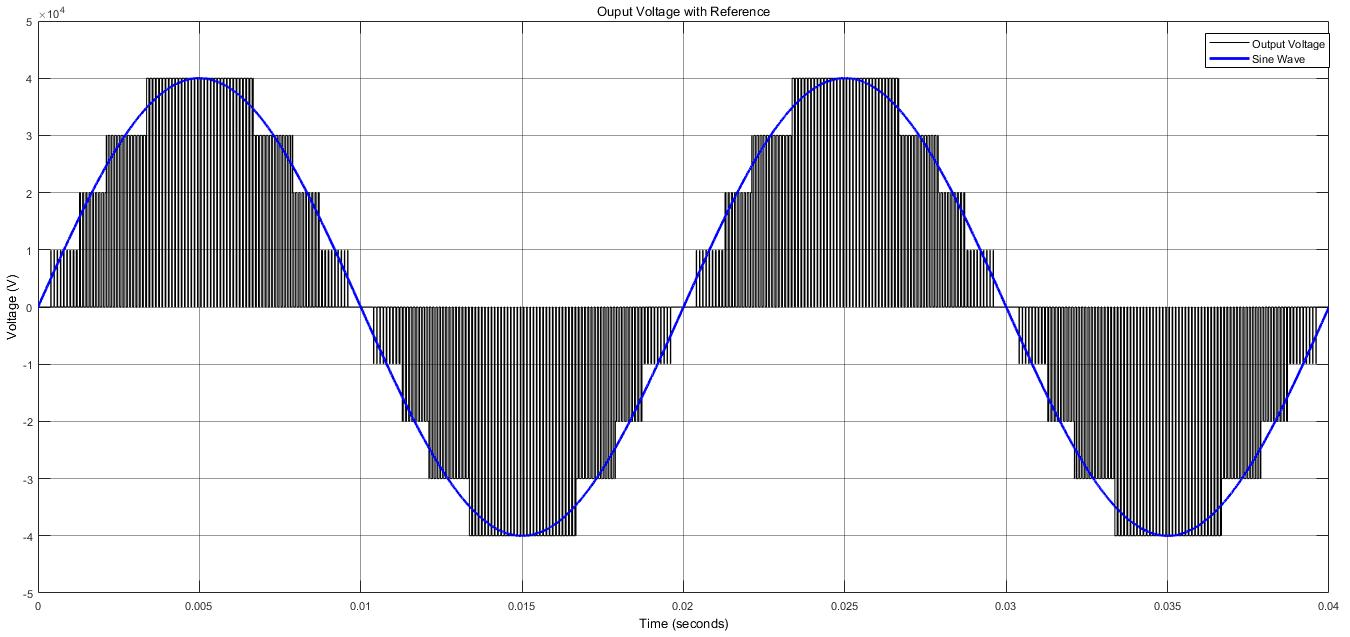
\includegraphics[width = 6in]{./Figures/Photos/Simulink/And_SPWM_Out.jpg}
	\rule{35em}{1pt}
	\caption{Output Signal after AND Operation}
\end{figure}

\begin{figure}[htbp]
	\centering
	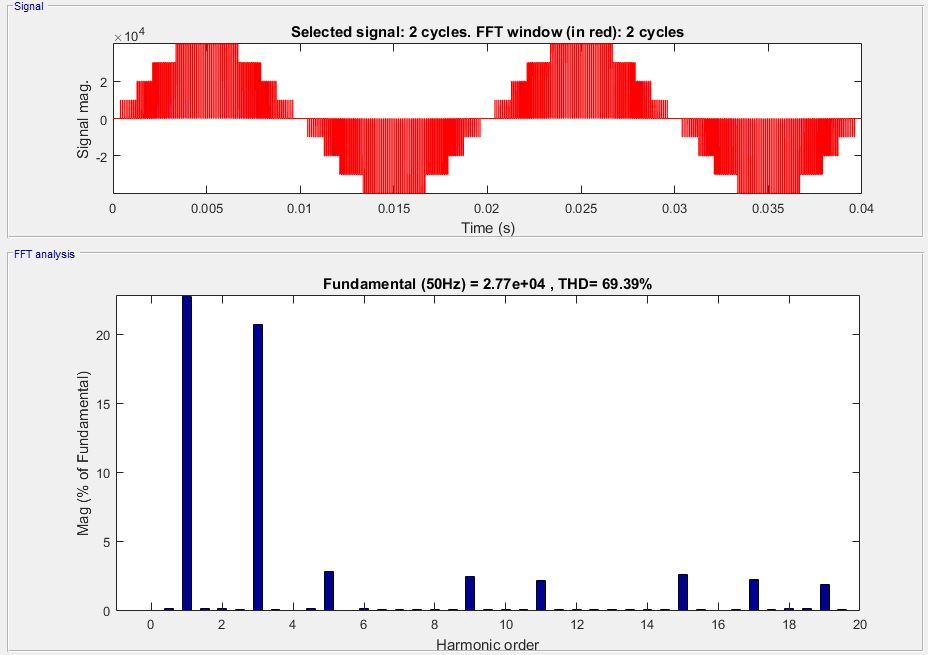
\includegraphics[width = 6in]{./Figures/Photos/Simulink/And_SPWM_Out_FFT.jpg}
	\rule{35em}{1pt}
	\caption{FFT of Output Signal after AND Operation}
\end{figure}

\section{SHE PWM}
Selective Harmonic Elimination is also very useful technique. For this project we have removed 5th, 7th and 13th harmonics form output waveform at 0.8 Modulation index. To do this we need to solve 4 non linear Equations:

\begin{equation}
cos(\alpha1) + cos(\alpha2) + cos(\alpha3) + cos(\alpha4) = 3.2
\end{equation}
\begin{equation}
cos(5\alpha1) + cos(5\alpha2) + cos(5\alpha3) + cos(5\alpha4) = 0
\end{equation}
\begin{equation}
cos(7\alpha1) + cos(7\alpha2) + cos(7\alpha3) + cos(7\alpha4) = 0
\end{equation}
\begin{equation}
cos(11\alpha1) + cos(11\alpha2) + cos(11\alpha3) + cos(11\alpha4) = 0
\end{equation}

\newpage
The previous conduction angles that was found by hit and trial method are:

\begin{center}
	\begin{tabular}{ |p{4cm}||p{4cm}|  }
		\hline
		\multicolumn{2}{|c|}{Conduction Angles} \\
		\hline
		Angle & Value in Degrees\\
		\hline
		$\alpha1$ & 6$^o$\\
		\hline
		$\alpha2$ & 22$^o$\\
		\hline
		$\alpha3$ & 38$^o$\\
		\hline
		$\alpha4$ & 60$^o$\\
		\hline
	\end{tabular}
\end{center}

By using fsolve command in MATLAB the following soltion is found. And the new conduction angles are:
 
 \begin{center}
 	\begin{tabular}{ |p{4cm}||p{4cm}|  }
 		\hline
 		\multicolumn{2}{|c|}{Conduction Angles for SHE PWM} \\
 		\hline
 		Angle & Value in Degrees\\
 		\hline
 		$\alpha1$ & 9.8409$^o$\\
 		\hline
 		$\alpha2$ & 20.3828$^o$\\
 		\hline
 		$\alpha3$ & 38.4054$^o$\\
 		\hline
 		$\alpha4$ & 60.4164$^o$\\
 		\hline
 	\end{tabular}
 \end{center}
 
 Below the results of SHE PWM are shown, it can be verified that the 5th, 7th and 11th harmonics are removed.
 
\begin{figure}[htbp]
	\centering
	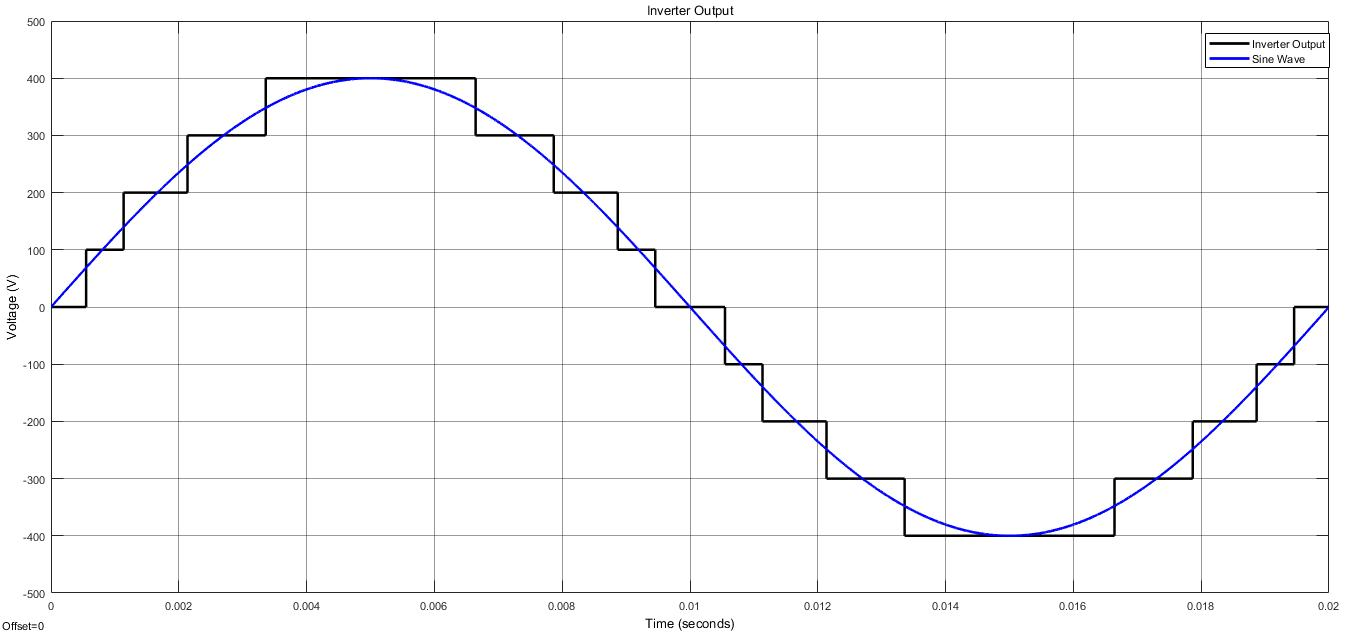
\includegraphics[width = 6in]{./Figures/Photos/Simulink/SHE_Out.jpg}
	\rule{35em}{1pt}
	\caption{Output Signal (SHE PWM)}
\end{figure}

\begin{figure}[htbp]
	\centering
	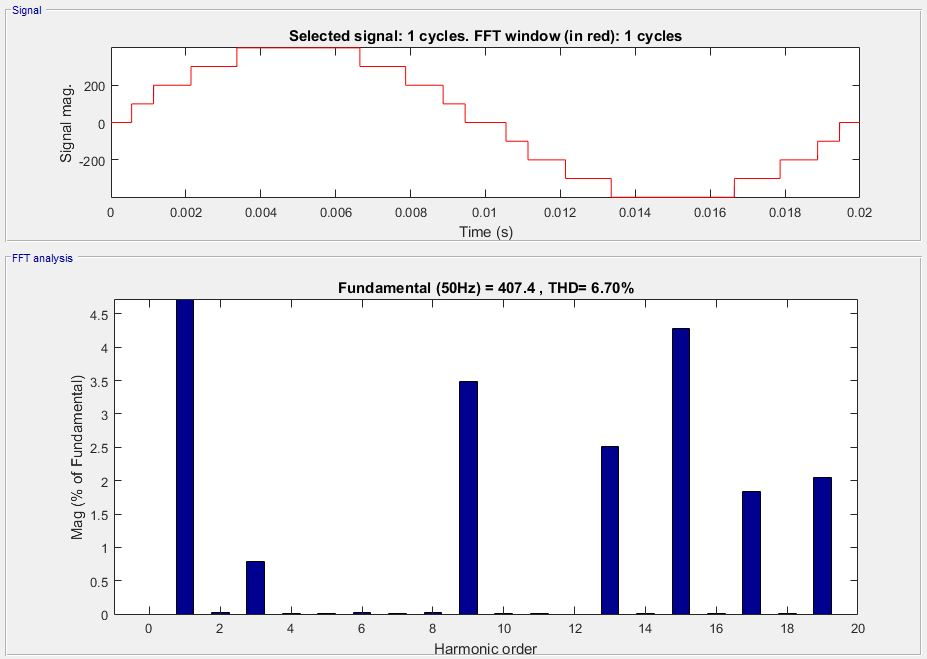
\includegraphics[width = 6in]{./Figures/Photos/Simulink/SHE_FFT.jpg}
	\rule{35em}{1pt}
	\caption{FFT of Output Signal (SHE PWM)}
\end{figure}
\begin{figure}[htbp]
	\centering
	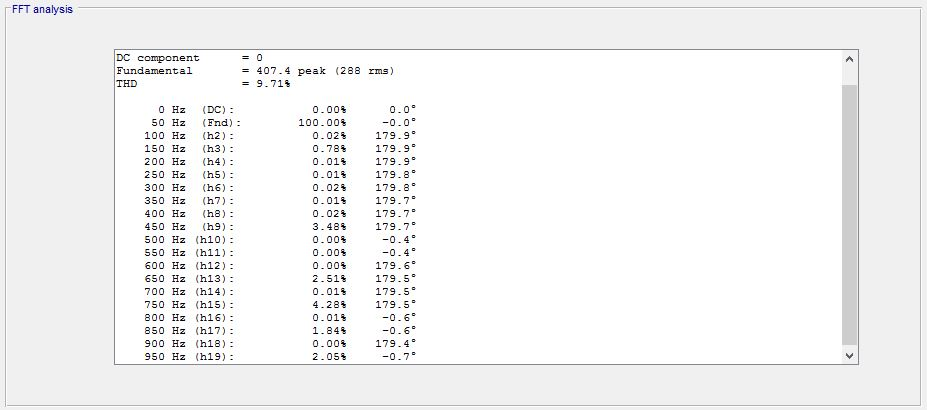
\includegraphics[width = 6in]{./Figures/Photos/Simulink/SHE_FFT_table.jpg}
	\rule{35em}{1pt}
	\caption{FFT Record Output Signal (SHE PWM)}
\end{figure}
\newpage
\section{Voltage Control}
We can control the value of RMS output voltage by taking AND operation of gating signals with a high frequency PWM signal. Then by changing the duty of PWM signal we can change the value of RMS output voltage.
Below is the relation between duty and V$_{rms}$:
 \begin{figure}[htbp]
 	\centering
 	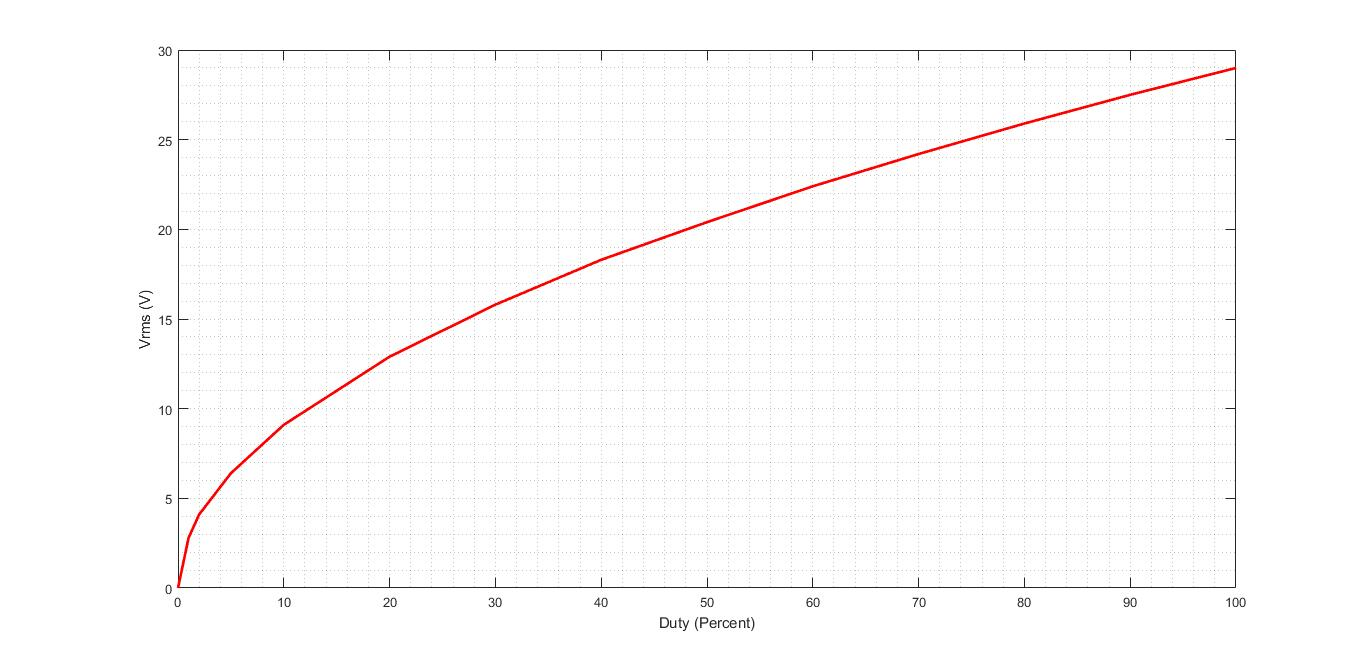
\includegraphics[width = 6in]{./Figures/Photos/Simulink/d_vrms.jpg}
 	\rule{35em}{1pt}
 	\caption{Relation between Duty Cycle of PWM and Vrms}
 \end{figure}
